\documentclass[reqno]{amsart}
\usepackage{geometry} 
\usepackage{amsmath}
\usepackage[super,sort&compress, comma]{natbib}
\usepackage{graphicx}
\usepackage{wrapfig}

\begin{document}

\title{Linked Selection Notebook}
\author{Jeremy Berg}
\date{}
\maketitle



\section*{Running Notes}

\begin{flushright}
	\textbf{November 20, 2012}
\end{flushright}

A sweep occurs yesterday $l$ base pairs away from a neutral site of interest. The probability that two randomly chosen lineages are forced to coalesce by the sweep is


$$\frac{1}{1 + \theta_b}e^{-\frac{1}{2}lr_{bp}T_{fix}}$$

where $r_{bp}$ is the recombination rate per base pair, $\theta_b$ is the population scaled mutation rate of beneficial mutations at the selected site, and $T_{fix}$ is the duration of the sweep in generations\cite{Pennings2006}. The $\frac{1}{1 + \theta_b}$ term is the probability neither lineage mutates off the selected background before coalescing, while $e^{-\frac{1}{2}lr_{bp}T_{fix}}$ is the probability that neither lineage recombines off the selected background during the course of the sweep.

Now, imagine that sweeps can occur at any base pair along the chromosome, and that they occur homogeneously along the chromosome, and through time, at a rate $\nu_{BP}$. Once again examining a single neutral locus, the rate at which recurrent, full, homogeneous soft sweeps force two lineages at the locus to coalesce is equal to


\begin{align}
	\lambda &= \nu_{BP}\frac{1}{1+\theta_b}\int_0^\infty e^{-\frac{1}{2}lr_{bp}T_{fix}}\mathrm d l\\
	& = \nu_{BP}\frac{1}{1+\theta_b}\left[\frac{1}{-\frac{1}{2}r_{bp}T_{fix}}e^{-\frac{1}{2}lr_{bp}T_{fix}}\right]_0^\infty \\
	&= \frac{2\nu_{BP}}{\left(1+\theta_b\right)r_{bp}T_{fix}}
\end{align}

The expectation of $\pi$ under this model is
\begin{align}
	\mathbb{E}\left[\pi\right] &= \frac{2\mu_n}{\frac{1}{2N} +  \frac{2\nu_{BP}}{\left(1+\theta_b\right)r_{bp}T_{fix}}} \\
	&= \frac{\theta_n}{1 + \frac{4N\nu_{BP}}{\left(1+\theta_b\right)r_{bp}T_{fix}}} \\
	& = \frac{r_{bp}\theta_n}{r_{bp} + \frac{4N\nu_{BP}}{\left(1+\theta_b\right)T_{fix}}}.
\end{align}
So $\frac{4N\nu_{BP}}{\left(1+\theta_b\right)T_{fix}}$ appears to be a big, messy, difficult to interpret compound parameter.

\newpage
\section*{Soft Sweeps from Mutation-Selection-Drift Balance.} 

\begin{flushright}
	\textbf{November 22, 2012}
\end{flushright}
To start, we'll just consider standing variation in a deterministic limit. We're interested in diversity at some neutral locus, which is some distance $l$ away from a selectively significant locus. Prior to some environmental change, mutations are deleterious with selection coefficient $s_d$, occur at rate $\mu_d$. Assuming $s_d>>\mu_d$, the frequency of deleterious alleles in the population is $\sim \frac{\mu_d}{s_d}$. As some point in time, a change in the environment occurs, causing this previously deleterious locus to become advantageous, and to sweep through the population. We are interested in the probability that this sweep forces two randomly chosen lineages at our neutral locus, $l$ base pairs away, to coalesce.

As with the recurrent mutation case above, the probability that the two lineages are forced to coalesce by a sweep that happened yesterday is
	$$Pr(\text{no recombination off sweep})Pr(\text{choose the same mutation class}).$$

\begin{flushright}
	\textbf{November 24, 2012}
\end{flushright}

Just as in the recurrent beneficial mutation example, 
\begin{equation}
	Pr(\text{no recombination off sweep}) = e^{-\frac{1}{2}lr_{bp}T_{fix}}
\end{equation}
where here I assume that the difference in $T_{fix}$ that results from the fact that the sweep begins at $\frac{\mu_d}{s_d}$ instead of $\frac{1}{2N}$ is negligible (and of course, sweep-like behavior doesn't actually begin at $\frac{1}{2N}$, but only once it gets to higher enough frequency to begin stochastic loss; probably, this all doesn't matter too much, but it'll be worth coming back to before publication). It conveniently turns out that, the sampling distribution for deleterious mutations at mutation-selection-drift balance is the Ewens sampling distribution,\cite{Ewens1972} where the $N$ in $\theta$ is replaced by $Nq$, where $q$ is the frequency of deleterious mutations in the population\cite{Hartl1982,Slatkin1997,Wakeley2008} (in this case $\frac{\mu_d}{s_d}$). Thus, 
\begin{equation}
	Pr(\text{choose the same mutation class}) = \frac{1}{1+\theta_{d,q}}
\end{equation}
where $\theta_{d,q} = 4N\frac{\mu_d}{s_d}\mu_d.$ As such,
\begin{align}
	Pr(\text{sweep forces coalescence}) = \frac{1}{1+\theta_{d,q}}e^{-\frac{1}{2}lr_{bp}T_{fix}}.
\end{align} 

Once again, envisioning a scenario where sweeps occur homogeneously across a chromosome of infinite length at rate $\nu_{BP}$, the total rate of coalescence at a site is

\begin{align}
	\lambda &= \frac{1}{2N}+\frac{\nu_{BP}}{1+\theta_{d,q}}\int_0^\infty e^{-\frac{1}{2}lr_{bp}T_{fix}}\mathrm d l\\
	&= \frac{1}{2N} + \frac{2\nu_{BP}}{\left(1+\theta_{d,q}\right)r_{bp}T_{fix}}.
\end{align}

The expectation of $\pi$ is thus
\begin{equation}
	\mathbb{E}\left[\pi\right] = \frac{r_{bp}\theta_n}{r_{bp} + \frac{4N\nu_{BP}}{\left(1+\theta_{d,q}\right)T_{fix}}}.
\end{equation}
The important insight is that, at least under certain assumptions, the effect of sweeps from standing, deleterious mutation on linked neutral diversity is essentially the same as that for sweeps from new, recurrent mutations, with the only different being the magnitude of the population scaled mutation rate parameter at the linked, non-neutral sites.

\begin{flushright}
	\textbf{November 25, 2012}
\end{flushright}

It seems like $\theta_{d,q}$ ought to be smaller than $\theta_b$ in most cases, and thus sweeps from recurrent beneficial mutation during the progress of the sweep ought to have a smaller effect on diversity than sweeps from standing deleterious variation.

\begin{flushright}
	\textbf{December 3, 2012}
\end{flushright}

It's been too long since my last entry. Need to get better about that.

First, it seems that my initial reading of the Hartl and Campbell paper\cite{Hartl1982} was a bit off. Their equations (2) and (9) together suggest that if one samples two lineages in the deleterious class, the probability that they are of the same type is
\begin{equation}
	Pr(k=1\mid n = 2 ) = \frac{1}{1+\theta_a}
\end{equation}
where $\theta_a = 4N\mu_a q_{eq}$. What I neglected was that their $\mu_a$ is not the same as the general mutation rate to a alleles. They define $\mu_a$ as follows:

\begin{equation}
	\mu_a = \frac{p\mu_{Aa} + q\mu_{aa}}{p\mu_{Aa} + q(1-\mu_{aA})}
\end{equation}
where $\mu_{ij}$ is the mutation rate from state i to state j. Roughly in parallel to the argument they put forward, if

\begin{align}
	\mu_{Aa}&=\mu_{aa}=\mu \\
	\mu_{aA} &= 0 \\ 
	&\text{and}, \notag\\
	q &= \frac{\mu}{s} \\
	&\text{then}, \notag\\
	\mu_a& = \frac{1}{1+\frac{1}{s}}	.
\end{align}

As 
\begin{equation}
	\theta_a = 4N\frac{\mu}{s}\frac{1}{1+\frac{1}{s}} = 4N\frac{\mu}{1+s}.
\end{equation}
Equations (13) and (19) together thus give us our probability of sampling two of the same type under mutation-selection drift balance. Of course, it turns out that for small $s$ this yields essentially the same value as the Hermisson and Pennings result\cite{Hermisson2005}. As $s$ grows larger, the Hartl and Campbell result returns a lower probability than the Hermisson and Pennings result. However, for most biologically plausible parameters, it seems like the results should be fairly close.

In the mean time, I've managed to write up a single locus Wright-Fisher simulation of an infinite alleles model for arbitrary mutation, selection, and population size parameters. It produces figures like this


\begin{flushleft}
	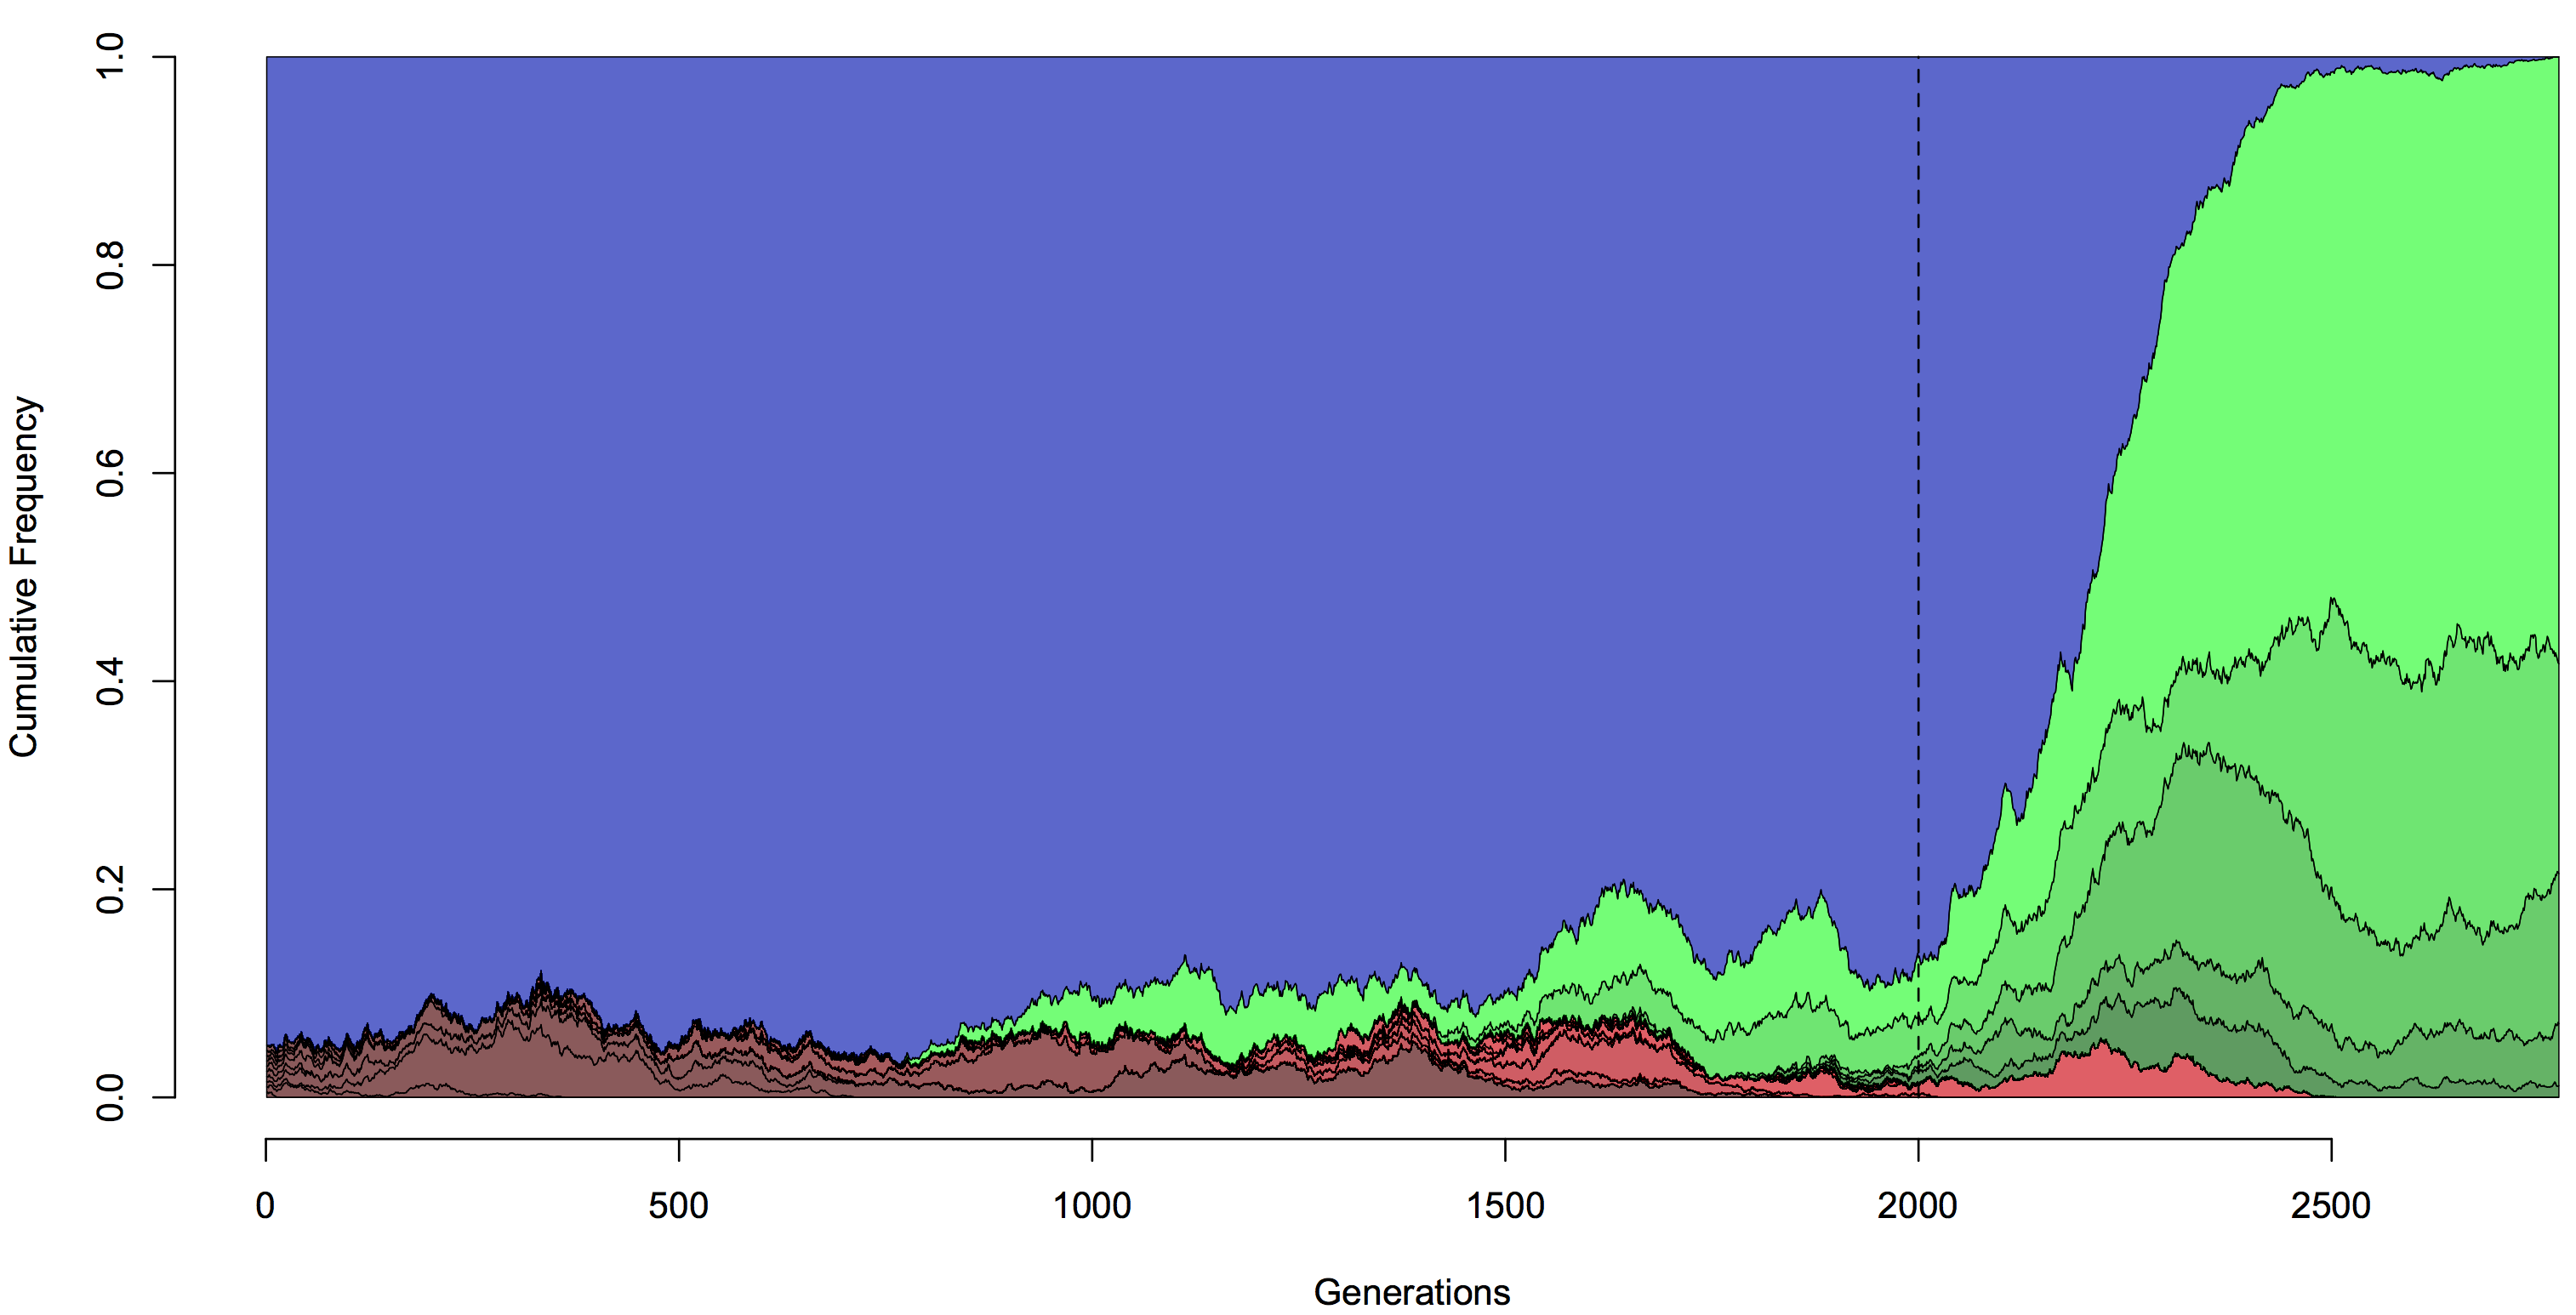
\includegraphics[width = \textwidth]{LSFigure1}
\end{flushleft}

This is a cumulative frequency plot, where each partition is a different independent mutation. Blue denotes the ancestral, neutral allele. Red and green mutations are selectively equivalent, the only difference being that the frequency trajectories of mutations that end up being members of the fixing class are colored green, while those that are lost before fixation are colored red. The dashed line denotes the point at which the mutation switches from being deleterious to beneficial.

These figures are pretty, but the real purpose is to use this simulation as a method of double checking my theoretical predictions.
\begin{flushright}
	\textbf{December 12, 2012}
\end{flushright}
In the past week or so we've managed to sort through some of this stuff and discover that my initial intuition, (which didn't even make it into the notebook because we got sidetracked by the Hartl and Campbell stuff) was correct. That is, as long as mutation continues during the course of the sweep (which is really the only biologically reasonable case, as there's no reason for mutation to stop once the sweep starts), then the Hermisson and Pennings result holds even if adaptation occurs from recurrent mutation to standing variation instead.

I had a chance to present the basic recurrent model at CoopIbarra this past Monday (and to chat with Michael yesterday morning), and folks who hadn't seen it yet seemed fairly receptive, and also pointed to working out the effect on linkage disequilibrium, or some other summary of haplotype structure. These results already exist for individual hard\cite{Stephan2006, McVean2007, Pfaffelhuber2008} and soft\cite{Pokalyuk2012} sweeps, so it seems like putting it into the recurrent model shouldn't be too hard.

\section*{The Relationship between Diversity and Population Size} 

\begin{flushright}
	\textbf{September 4, 2013}
\end{flushright}
We'll begin from the recurrent soft sweep result above, namely the observation that
\begin{align}
	\lambda = \frac{1}{2N} + \frac{2\nu}{\left(1+\theta_b\right)r_{bp}T_{fix}}.
\end{align}
Next, assume $N$ is very large, such that $\theta_b = 4N\mu_b>>1$, and thus we can safely ignore the 1 and let
\begin{align}
	\lambda = \frac{1}{2N} + \frac{2\nu}{4N\mu_br_{bp}T_{fix}}.\label{coal.rate}
\end{align}
We want to consider the effect of recurrent soft sweeps on neutral genetic diversity, but we don't want to land in the Desai/Neher (fitness class coalescent) world\cite{Desai:2007fh,Desai:2013tk,Neher:2013wu,Neher:2013il}, where new beneficial mutations occur on the background of the last beneficial mutation before it has managed to fix. We need the rate of sweeps to be slow enough that the previous sweep has managed to fix before the next comes along. We can ensure that we are in this parameter range by considering that the waiting time until the next sweep (starting from the beginning of the last one) can be written as
\begin{align}
	\frac{1}{\nu} = \frac{1}{\alpha} + \frac{1}{2N\mu_b s}
\end{align}
where $\alpha$ describes the rate of ecological necessity (i.e. the rate at which the environment changes such that new mutations will be beneficial; they are assumed deleterious or neutral in the intervening time). We can then solve for 
\begin{align}
	\nu = \frac{2N\mu_b s \alpha}{2N\mu_bs + \alpha}
\end{align}

Because the population size is large enough to be generating predominantly soft sweeps, but the environment changes rather infrequently, we can assume $2N\mu_bs >> \alpha$, and thus simply take $\nu=\alpha$. It is also worth noting that because $s = \frac{log(2Ns)}{T}$, we can rewrite our assumption as 
\begin{align}
	\frac{2N\mu_b log(2Ns)}{T} >> \alpha
\end{align}
and then multiple both sides by $\frac{1}{T}$ to get
\begin{align}
	\frac{2N\mu_b log(2Ns)}{T^2} >> \frac{\alpha}{T}.
\end{align}
This sets an upper bound on the value of $\frac{\alpha}{T}$, but we can do one better. To make things easy, assume that the rate of ecological change is sufficiently slow relative to the duration of the sweeps, such that the next sweep cannot begin until the previous one has fixed
\begin{align}
	\frac{1}{\alpha} > T
\end{align}
which we can rewrite as
\begin{align}
	\frac{1}{T^2}>\frac{\alpha}{T}
\end{align}
thus setting an upper bound on $\frac{\alpha}{T}$.

Now, we rewrite \eqref{coal.rate} as 
\begin{align}
	\lambda = \frac{1}{2N} + \frac{2\alpha}{4N\mu_br_{bp}T}
\end{align}
and therefore note that
\begin{align}
	\pi &= \frac{2\mu_n}{\frac{1}{2N} + \frac{2\alpha}{4N\mu_br_{bp}T}}\\
	&= \frac{4N\mu_n}{1 + \frac{\alpha}{\mu_b r T}}\\
	&= \frac{4N\mu_n}{1 + \frac{\alpha}{T}\frac{1}{\mu_b r}}.
\end{align}
We can restate our assumption $\frac{1}{T^2} > \frac{\alpha}{T}$ as
\begin{align}
	\frac{T}{\alpha} > T^2.
\end{align}

We find that coalescence is dominated by drift when $\frac{1}{\mu_b r} << \frac{T}{\alpha} \approx T^2$ (resulting in $\pi \approx 4N\mu_n$), and by sweeps when $\frac{1}{\mu_b r} >> \frac{T}{\alpha} \approx T^2$ in which case 
\begin{align}
	\pi \approx \frac{4NT\mu_n\mu_b r_{bp}}{\alpha}
\end{align}
and the transition between the two parameter regimes occurs roughly when $\frac{1}{\mu_b r} \approx T^2$. 

Just to get a rough sense of where this puts us, if sweeps are occurring in a population of $N = 1,000,000$ with $s=10^{-5}$ ($2Ns = 20$), and $r_{bp} = 10^{-8}$, then drift dominates if $\mu_{b}>>10^{-3}$ (because sweeps are so soft that they hardly force any coalescence), while draft dominates if $\mu_b<<10^{-3}$. If instead $s=10^{-4}$, then $\mu_b>>10^{-2}$ in order for drift to dominate, while at $s=10^{-3}$ the mutation rate would have to be greater than one in order for drift to dominate. 

These calculations assume that $\alpha$ is near its maximum value of $\sim\frac{1}{T}$. As $\alpha$ decreases, so too must $\mu_b$ in order for sweeps to continue to dominate coalescence. Eventually, of course, this approximation breaks down because the sweeps start to become predominantly hard (i.e. $4N\mu_b < 1$). Many things seem to happen at once here, as we also reach the point at which $\nu = \alpha$ is no longer a valid approximation either (because the waiting time for a new mutation becomes non-negligible). It seems like these should happen at roughly the same time, but I haven't worked through that yet.

\section*{Sweeps From IBD Standing Variation} 
\begin{flushright}
	\textbf{December 12, 2012}
\end{flushright}

It also seems like we might relatively easily be able to make progress on the hard sweep from IBD standing variation case, and that once this is done we should be able to include these sort of sweeps in a general recurrent model. Graham sent me a few papers about the conditional genealogy of a sample in which a subset of chromosomes are observed to carry a particular mutation, notably one from Griffiths and Tavar{\'e}\cite{GriffithsTavare:2003}, and this seems significant enough, with enough of a clear way forward that I'm going to create a separate entry here.

Another really useful thing to do might be to work out the sampling formula for the number of haplotypes as a function of the recombination distance from the sweeping locus (which we suspect should have a roughly Ewens like distribution, with the $\theta$ parameter given by something like $2Nrf$, where $r$ is the recombination rate, while $f$ is the frequency from which the sweep started), and then develop a likelihood framework to infer $f$ from the haplotype structure on either side of the sweep.

In addition to this analytical work, another objective is going to be writing out a structured coalescent simulation on a sweeping background, probably using Graham and Molly's trick from 2005\cite{Przeworski2005} to simulate the trajectory of the sweeping allele, and then just run coalescent simulations under that background.

\begin{flushright}
	\textbf{February 4, 2012}
\end{flushright}

The simulation is pretty much written. More on that later hopefully. At present, the problem is this: 

Assuming a sample of three lineages, what is the probability that there are 2 different haplotypes at a distance from the selected site of $l_1$, given that there is only one haplotype at a distance of $l_1-1$. If $b_1$, $b_2$ and $b_3$ are the external branches of the tree, and $b_4$ is the one internal branch, then
\begin{align}
	& P(\text{2 haplotypes at } l_1 \mid  \text{1 haplotype at } l_1-1) = \\
	& P(\text{rec before } \tau \text{ and no rec on other two lineages before they coalesce}) + \\
	& P(\text{no rec before }\tau \text{, then rec after } \tau \text{ but before coalescence})
\end{align}
where $\tau$ is the point in time at which the other two lineages coalesce with one another (conditional on previous base assumed and dropped from here out).

First recognize that
\begin{align}
	& P(\text{rec before } \tau \text{, then no rec on other two lineages before they coalesce}) = \\
	& P(\text{rec before } \tau)P(\text{no rec on other two lineages before they coalesce})
\end{align}
\begin{align}
	P(\text{rec before } \tau)&= \int_0^\infty 3r (1-f) \mathrm{e}^{-3tr(1-f)}\mathrm{e}^{-\frac{t\binom{3}{2}}{2N_ef}}\, \mathrm{d} t \\
	& = \frac{3r (1-f)}{3r(1-f) + \frac{3}{2N_ef}} \\
	& = \frac{6N_e r (1 -f )}{6N_e r f (1 -f ) + 3} \\
	& = \frac{4N_e r f (1 -f )}{4N_e r f (1 -f ) + 2}
\end{align}
\begin{align}
	P(\text{no rec on other two lineages before they coalesce}) & = \int_0^\infty\frac{1}{2N_ef}\mathrm{e}^{-2tr(1-f)}\mathrm{e}^{-\frac{t}{2N_e f}}\, \mathrm{d}t \\ 
	& = \frac{\frac{1}{2N_ef}}{2r(1-f) + \frac{1}{2N_e f}} \\
	& = \frac{1}{4Nrf(1-f) + 1}
\end{align}
So,
\begin{align}
	P(\text{rec before } \tau \text{, then no rec on other two lineages before they coalesce}) = \\
	\left(\frac{1}{4Nrf(1-f) + 1}\right)\left(\frac{4N_e r f (1 -f )}{4N_e r f (1 -f ) + 2}\right)
\end{align}
Next
\begin{align}
	 P(\text{no rec before }\tau \text{, then rec after } \tau \text{ but before coalescence})= \\
	 P(\text{rec after } \tau \text{ but before coalescence} \mid \text{no rec before }\tau)P(\text{no rec before }\tau )
\end{align}
\begin{align}
P(\text{no rec before }\tau ) & = \int_0^\infty\frac{\binom{3}{2}}{2N_e f}\mathrm{e}^{-3r(1-f)}\mathrm{e}^{-\frac{t\binom{3}{2}}{2N_e f}}\, \mathrm{d} t\\
	& =\frac{\frac{3}{2N_e f}}{3r(1-f) + \frac{3}{2N_e f}} \\
	& = \frac{3}{6N_erf(1-f) + 3} \\
	& = \frac{2}{4N_erf(1-f) + 2}
\end{align}
\begin{align}
	P(\text{rec after } \tau &\text{ but before coalescence} \mid \text{no rec before }\tau) = \\
	& = \int_0^\infty2r(1-f)\mathrm{e}^{-2r(1-f)}\mathrm{e}^{-\frac{-t}{2N_ef}}\, \mathrm{d}t \\
	& = \frac{2r(1-f)}{2r(1-f)+\frac{1}{2N_e f}} \\
	& = \frac{4N_e r f (1-f)}{4N_e r f (1-f) + 1}
\end{align}
So,
\begin{align}
	P(\text{no rec before }\tau \text{, then rec after } \tau \text{ but before coalescence}) = \\
	\left(\frac{2}{4N_erf(1-f) + 2}\right)\left(\frac{4N_e r f (1-f)}{4N_e r f (1-f) + 1}\right)
\end{align}
Letting $R_f = 4N_e r f (1-f)$, then
\begin{align}
	P(\text{2 haplotypes at } l_1 \mid  \text{1 haplotype at } l_1-1) = \\
	\frac{R_f}{R_f+2}\frac{1}{R_f+1} + \frac{2}{R_f + 2}\frac{R_f}{R_f+1} \\
	= \frac{3R_f}{(R_f+2)(R_f+1)}
\end{align}
which is the Ewens Sampling result for $P(k=2\mid n=3,R_f)$, where $R_f$ is filling the role of $\theta$.

\newpage
\begin{flushright}
	\textbf{February 5, 2013}
\end{flushright}

Now I'm going to move on to thinking about the probability of having a recombination event that increased the number of haplotypes from 1 to 2 at $l_1$, followed by a recombination event that increases the number of haplotypes from 2 to 3 at $l_2$, where $l_1 < l_2$ are distances in base pairs from the selected site. In other words

\begin{align}
	& P(\{3\} \rightarrow \{2,1\} \text{ at } l_1 \text{ and } \{2,1\} \rightarrow \{1,1,1\} \text{ at } l_2) = \\
	& P(\{l_1b_3\} \text{ and} \left\{\{l_2b_1\} \text{ or } \{l_2b_2\}\right\}) + \\
	& P(\{l_1b_4\} \text{ and} \left\{\{l_2b_1\} \text{ or } \{l_2b_2\}\right\}) + \\
	& P(\{l_1b_5\} \text{ and} \left\{\{l_2b_1\} \text{ or } \{l_2b_2\}\right\}) + \\
	& P(\{l_2b_3\} \text{ and} \left\{\{l_1b_1\} \text{ or } \{l_1b_2\}\right\}) + \\
	& P(\{l_2b_4\} \text{ and} \left\{\{l_1b_1\} \text{ or } \{l_1b_2\}\right\}) + \\
	& P(\{l_2b_5\} \text{ and} \left\{\{l_1b_1\} \text{ or } \{l_1b_2\}\right\})
\end{align}
where $b_1$ and $b_2$ are the branches connecting two of the tips to the first coalescent event, which occurs at $\tau_2$ (the first moment when there are two ancestors of the sample), $b_3$ is the branch from the third tip leading back to time $\tau_2$, $b_4$ is contiguous with $b_3$ and leads from $\tau_2$ back to $\tau_1$, where it coalesces with $b_5$, which is the branch subtending $b_1$ and $b_2$; $l_ib_j$ is a recombination event occurring at sequence location $i$ on branch $j$. Moving forward
\begin{align}
	& P(\{l_1b_3\} \text{ and} \left\{\{l_2b_1\} \text{ or } \{l_2b_2\}\right\}) = \\
	& P(\{l_1 b_3\}, \text{then} \left\{\{l_2 b_1\} \text{ or } \{l_2 b_2\}\right\}, \text{then } \{b_1\text{ and } b_2 \text{ coalesce}\}, \text{then } \{b_4 \text{ and } b_5 \text{ coalesce}\}) + \\
	& P(\left\{\{l_2 b_1\} \text{ or } \{l_2 b_2\}\right\}, \text{then } \{l_1 b_3\}, \text{then } \{b_1\text{ and } b_2 \text{ coalesce}\}, \text{then } \{b_4 \text{ and } b_5 \text{ coalesce}\})
\end{align}
These two events have equal probability and thus
\begin{align}
		& P(\{l_1b_3\} \text{ and} \left\{\{l_2b_1\} \text{ or } \{l_2b_2\}\right\}) = \\
		& 2P(\{l_1 b_3\}, \text{then} \left\{\{l_2 b_1\} \text{ or } \{l_2 b_2\}\right\}, \text{then } \{b_1\text{ and } b_2 \text{ coalesce}\}, \text{then } \{b_4 \text{ and } b_5 \text{ coalesce}\})
\end{align}
\begin{align}
& P(\{l_1 b_3\}, \text{then} \left\{\{l_2 b_1\} \text{ or } \{l_2 b_2\}\right\}, \text{then } \{b_1\text{ and } b_2 \text{ coalesce}\}, \text{then } \{b_4 \text{ and } b_5 \text{ coalesce}\})  = \\
& r(1-f)\int_0^\infty \mathrm{e}^{-t r l_1 ( 1-f )} \mathrm{e}^{ -2 t r l_2 ( 1-f ) } \mathrm{e}^{-\frac{t\binom{3}{2}}{2 N_e f}}\, \mathrm{d}t \\
	& 2 r (1-f) \int_0^\infty \mathrm{e}^{-t r l_1 ( 1-f )} \mathrm{e}^{ -2 t r l_2 ( 1-f ) } \mathrm{e}^{-\frac{t\binom{3}{2}}{2 N_e f}}\, \mathrm{d}t \\ 
	& \frac{1}{2 N_e f}\int_0^\infty \mathrm{e}^{-t r l_1 ( 1-f )} \mathrm{e}^{ -2 t r l_2 ( 1-f ) } \mathrm{e}^{-\frac{t\binom{3}{2}}{2 N_e f}}\, \mathrm{d}t \\
	& \frac{1}{2 N_e f}\int_0^\infty \mathrm{e}^{-t r l_1 ( 1-f )} \mathrm{e}^{ - t r l_2 ( 1-f ) } \mathrm{e}^{-\frac{t}{2 N_e f}}\, \mathrm{d}t = \\
	& \frac{\left[2N_erf(1-f)\right]\left[4N_erf(1-f)\right]\left[1\right]\left[1\right]}{\left[2N_erf(1-f)l_1 + 2N_erf(1-f)l_2+3\right]^3\left[2N_erf(1-f)l_1 + 2N_erf(1-f)l_2 + 1\right]}
\end{align}

Letting $R_f = 2N_erf(1-f)$, we can write down
\begin{equation}
P(l_1b_3,l_2b_1 \text{ or } l_2b_2) = \frac{4R_f^2}{\left(R_f l_1 + 2R_f l_2 + 3\right)^3\left(R_f\left(l_1 + l_2\right) + 1 \right)}
\end{equation}

Next
\begin{align}
	& P(\{l_1b_4\} \text{ and} \left\{\{l_2b_1\} \text{ or } \{l_2b_2\}\right\}) = \\
	& P(\left\{\{l_2 b_1\} \text{ or } \{l_2 b_2\}\right\}, \text{then} \left\{b_1 \text{ and } b_2 \text{ coalesce}\right\}, \text {then } \{l_1b_4\}, \text{then} \left\{b_4 \text{ and } b_5 \text{ coalesce} \right\}) = \\
	& 2r(1-f) \int_0^\infty \mathrm{e}^{-trl_1(1-f)}\mathrm{e}^{-2trl_2(1-f)}\mathrm{e}^{-\frac{t\binom{3}{2}}{2N_ef}}\mathrm{d}t \\
	& \frac{1}{2N_ef} \int_0^\infty \mathrm{e}^{-trl_1(1-f)}\mathrm{e}^{-2trl_2(1-f)}\mathrm{e}^{-\frac{t\binom{3}{2}}{2N_ef}}\mathrm{d}t \\
	& r(1-f) \int_0^\infty \mathrm{e}^{-trl_1(1-f)}\mathrm{e}^{-trl_2(1-f)}\mathrm{e}^{-\frac{t}{2N_ef}}\mathrm{d}t \\
	& \frac{1}{2N_ef} \int_0^\infty \mathrm{e}^{-trl_1(1-f)}\mathrm{e}^{-trl_2(1-f)}\mathrm{e}^{-\frac{t}{2N_ef}}\mathrm{d}t = \\
	& \frac{\left[2r(1-f)\right]\left[\frac{1}{2N_ef}\right]^2\left[r(1-f)\right]}{\left[rl_1 (1-f) + 2r l_2 (1-f) + \frac{3}{2N_ef}\right]^2\left[r l_1 (1-f) + r l_2 (1-f) + \frac{1}{2N_e f} \right]^2}
\end{align}
Again, multiplying top and bottom by $\left(2N_ef\right)^4$, and letting $R_f = 2N_erf(1-f)$
\begin{equation}
	P(\{l_1b_4\} \text{ and} \left\{\{l_2b_1\} \text{ or } \{l_2b_2\}\right\}) = \frac{2R_f^2}{\left(R_f l_1 + 2R_f l_2 + 3\right)^2\left(R_f l_1 + R_f l_2 + 1\right)^2}
\end{equation}

Next (now omitting the integrals for brevity's sake)
\begin{align}
	& P(\{l_1b_5\} \text{ and} \left\{\{l_2b_1\} \text{ or } \{l_2b_2\}\right\}) = \\
	& P(\left\{\{l_2 b_1\} \text{ or } \{l_2 b_2\}\right\}, \text{then} \left\{b_1 \text{ and } b_2 \text{ coalesce}\right\}, \text {then } \{l_1b_5\}, \text{then} \left\{b_4 \text{ and } b_5 \text{ coalesce} \right\}) = \\
	& \left[\frac{2r(1-f)}{3rl_2(1-f) + \frac{3}{2N_ef}}\right] \left[\frac{\frac{1}{2N_ef}}{3rl_2(1-f) + \frac{3}{2N_ef}}\right] \left[\frac{r(1-f)}{2rl_2(1-f) + \frac{1}{2N_ef}}\right] \left[\frac{\frac{1}{2N_ef}}{2rl_2(1-f) + \frac{1}{2N_ef}}\right] = \\
	& \frac{2R_f^2}{\left(3R_f l_2 + 3\right)^2\left(2R_f l_2 + 1 \right)^2}
\end{align}
and if we carry out the same calculation for $P(\left\{\{l_1b_1\} \text{ or } \{l_1b_2\}\right\} \text{ and} \{l_2b_5\})$, we find that it is equivalent to the calculation we just carried out for $P(\{l_1b_5\} \text{ and} \left\{\{l_2b_1\} \text{ or } \{l_2b_2\}\right\})$ (which makes sense if you squint at the tree a bit).

\begin{flushright}
	\textbf{September 3, 2013}
\end{flushright}

Ok! Been a while since I've written anything here. Polygenic selection paper is up on arXiv and submitted to PLoS Genetics, so time to get back to sweep work. While variations of the above can in principle be used to infer the frequency parameter, we now live in a world where direct inference of the distribution of ARGs from sequence data seems to be possible\cite{Rasmussen:2013wv}, and thus it may be worth considering how to do this inference problem if we get to know the coalescent times at the selected site.

Imagine we have an allele that begins at frequency $f$ (having been neutral before that), and sweeps with strength $s$ in a population of size $N$. Consider then sampling $n$ lineages at $t=0$ (the present), and following them backward in time. To a first approximation, no coalescence occurs during the sweep, and thus we might imagine that we could write down a likelihood function that looks like

\begin{align}
	\mathcal{L}(s,f\mid \vec{\tau}) = \left(\frac{1}{Nf}\right)^{n-1} e^{-\frac{\binom{n}{2}}{Nf}\left(\tau_1 - \tau_s\right)}\prod_{i=2}^{n-i+1}e^{-\frac{\binom{n-i+1}{2}}{Nf}\left(\tau_i-\tau_{i-1}\right)}
\end{align}
where $\tau_s = \frac{ln(N\frac{1-f}{f})}{s}$ is the number of generations (backward in time) that it take for the sweep to go from fixation down to frequency $f$.

Unfortunately, coalescence can occur during the sweep, and thus by completely prohibiting it in our likelihood function, we could find ourselves in situations where we have no choice but to infer totally ridiculous selection coefficients, simply because that's the only way that we can have $\tau_s<\tau_1$.

Alternatively, if we allow coalescence during the sweep, we can make the assumption that the frequency path is deterministic, and thus use that to get coalescence probabilities in each generation. We take the number of beneficial alleles present in generation $t$ (before the present) to be a deterministic function of $s$ and $t$
\begin{align}
	N(t) = N - \frac{N e^{st}}{N-1+e^{st}} 
\end{align}
where $N$ is the population size. If, for example, we have a single coalescent event that occurs at $t=\tau_1<\tau_s$, then we can calculate the probability of that coalescent event occurring during the sweep as 
\begin{align}
	\frac{1}{N(\tau_1)}e^{-\binom{n}{2}\int_0^{\tau_1}\frac{1}{N(t)}dt}
\end{align}
where
\begin{align}
	\int\frac{1}{N(t)}dt = \int\frac{1}{N - \frac{Ne^{st}}{N - 1 + e^{st}}}dt = \frac{e^{st}}{\left(N-1\right)Ns} + \frac{t}{N} + C.
\end{align}
We then need to prohibit coalescence from $\tau_1$ to $\tau_s$, and then start running the standard coalescent at rate $\frac{1}{Nf}$
\begin{align}
	\left(\frac{1}{Nf}\right)^{n-2}e^{-\binom{n-1}{2}\left(\int_{\tau_1}^{\tau_s}\frac{1}{N(t)}dt-\frac{1}{Nf}\left(\tau_2-\tau_{s}\right)\right)}\prod_{i=3}^{n-i+1}e^{-\frac{\binom{n-i+1}{2}}{Nf}\left(\tau_i-\tau_{i-1}\right)}
\end{align}
and thus the full likelihood can be written as
\begin{align}
	\mathcal{L}(s,f\mid \vec{\tau})=\frac{1}{N(\tau_1)}e^{-\binom{n}{2}\int_0^{\tau_1}\frac{1}{N(t)}dt}\left(\frac{1}{Nf}\right)^{n-2}e^{-\binom{n-1}{2}\left(\int_{\tau_1}^{\tau_s}\frac{1}{N(t)}dt-\frac{1}{Nf}\left(\tau_2-\tau_{s}\right)\right)}\prod_{i=3}^{n-i+1}e^{-\frac{\binom{n-i+1}{2}}{Nf}\left(\tau_i-\tau_{i-1}\right)}.
\end{align}

In this example, we've imagined that only one coalescent event occurs during the sweep, but in practice it is possible that more than one could (particularly if we are evaluating the likelihood for a fairly small $s$), in which case we simply include terms such as $\frac{1}{N(\tau_2)}e^{-\binom{n-1}{2}\int_{\tau_1}^{\tau_2}\frac{1}{N(t)}dt}$, and take the product for the neutral phase starting with $i=4$, etc.

\begin{flushright}
	\textbf{September 13, 2013}
\end{flushright}

Consider now a case where a selectively neutral allele arises in some ancestral population and drifts up to some frequency $f$. Individuals from this ancestral population then go on to found multiple independent populations in some new environment. A bottleneck occurs for some number of generations during the founding event, after which the previously neutral mutation is becomes beneficial in all of the new environments. The biological model one should have in mind is something like Sticklebacks colonizing lakes and streams in British Columbia, or Mimulus on heavy metal soils in California.

We'll generally focus on pairwise quantities here, although thinking about the joint AFS later on may be interesting. One useful thing to consider is the expectation of $F_{ST}$ between two of the founder populations as we move away from the selected site. Consider that $F_{ST}$ can be expressed as
\begin{align}
	F_{ST} = \frac{T_T - T_S}{T_T}
\end{align}
where $T_T$ is the average pairwise coalescence time of a pair of lineages sampled randomly from the two founder populations, and $T_S$ is the average pairwise coalescence time of two lineages sampled from the same population.

If $T_D$ is the average pairwise coalescence time of two lineages sampled from different populations, then because sampling two lineages randomly from the total population results in a $50\%$ chance of sampling lineages from the same population, and $50\%$ chance of sampling from different populations, $T_T = \frac{T_D + T_S}{2}$. Therefore
\begin{align}
	F_{ST} = \frac{\frac{T_D+T_S}{2} - T_S}{\frac{T_D+T_S}{2}} &= \frac{T_D+T_S - 2T_S}{T_D+T_S} \\
	&= \frac{T_D - T_S}{T_D + T_S}
\end{align}
and so if we can simply write down expectations for $T_D$ and $T_S$ in terms of relevant parameters, then we can get an expression describing the expected value of $F_{ST}$ as a function of distance from the recombination site and other relevant population genetic parameters.
\begin{flushright}
	\textbf{October 2, 2013}
\end{flushright}
\begin{align}
	T_S = &P(\text{rec out during sweep}) \mathbb{E}[T_2] + \\
	&P(\text{no rec out during sweep})P(\text{rec out during bottleneck before coal})\mathbb{E}[T_2] \\
	&P(\text{no rec out during sweep})P(\text{no rec out or coal during bottleneck})\\&P(\text{ancestral rec before coal})\mathbb{E}[T_2]
\end{align}
or, for shorthand, if $P_{S,S}$ is the probability of a recombination event happening during the sweep, $P_{B,S}$ the probability of recombining before coalescing during the bottleneck, $P_{EB,S}$ is the probability of escaping the bottleneck without recombining or coalescing, and $P_{A,S}$ the probability of recombining before coalescing during the ancestral phase, then
\begin{align}
	T_S = &P_{S} \mathbb{E}[T_2] + (1-P_{S})P_{B,S}\mathbb{E}[T_2] + (1-P_{S})P_{EB,S}P_{A}\mathbb{E}[T_2].
\end{align}
In contrast, when considering expected coalescent time of two sequences sampled from different populations
\begin{align}
	T_D = P(\text{rec during sweep})\mathbb{E}[T_2] + P(\text{no rec in sweep})P(\text{rec in bottleneck})\mathbb{E}[T_2] +\\
	P(\text{no rec in sweep})P(\text{no rec bottleneck})P(\text{rec ancestral})\mathbb{E}[T_2]
\end{align}
or
\begin{align}
	T_D = P_{S} \mathbb{E}[T_2] + (1-P_{S})P_{B,D}\mathbb{E}[T_2] + (1-P_{S})(1-P_{B,D})P_{A}\mathbb{E}[T_2].
\end{align}
Plugging in to our expression above, we find that the numerator can be written as
\begin{align}
	(1-P_S)[P_{B,D} - P_{B,S} + P_A(1- P_{B,D} - P_{EB,S})]\mathbb{E}[T_2],
\end{align}
and the denominator as
\begin{align}
	2P_S + (1-P_S)[(1-P_A)P_{B,D} + P_{B,S} + P_A(1 + P_{EB,S})]\mathbb{E}[T_2].
\end{align}
Our expression for $F_{ST}$ is thus
\begin{align}
	F_{ST} = \frac{(1-P_S)[P_{B,D} - P_{B,S} + P_A(1- P_{B,D} - P_{EB,S})]}{2P_S + (1-P_S)[(1-P_A)P_{B,D} + P_{B,S} + P_A(1 + P_{EB,S})]}.
\end{align}
From previous work above, we have
\begin{align}
	P_A &= \frac{R_f}{1+R_f} \\
	P_S &= 1 - e^{-2r\int_0^{T_{\text{fix}}}1-X(t)\mathrm{d}t} \\
	\text{while}\\
	P_{B,D} &= 1-  e^{-2rT_{bot}(1-f)} \\
	P_{B,S} &= r(1-f)\int_0^{T_{bot}}e^{-2tr(1-f)}e^{-\frac{t}{2NfB}}\mathrm{d}t\\
	P_{EB,S} &= e^{-2T_{bot}r(1-f)-\frac{T_{bot}}{2NfB}}
\end{align}

Alternatively, there's a bottleneck that happens at exactly the same time the sweep starts, but we've taken our sample some number of generations after the sweep has finished. Thus, if $P_C$ is the probability that two lineages sampled from the same population coalesce before the sweep starts, we throw out all of the $P_{B,--}$ terms, and keep everything else, then
\begin{align}
	T_S &= (1-P_C)P_S + (1-P_C)(1-P_S)P_A \\
	T_D &= P_S + (1-P_S)P_A \\
	F_{ST} &= \frac{P_S\left(P_A + P_C - P_A P_C\right)}{\left(2-P_C\right)\left(P_S + P_A - P_S P_A\right)} 
\end{align}
where again
\begin{align}
	P_A &= \frac{R_f}{1+R_f} \\
	P_S &= 1 - e^{-2r\int_0^{T_{\text{fix}}}1-X(t)\mathrm{d}t} \\
	&\text{and} \\
	P_C & = \frac{1}{2NB}e^{-\frac{T_0}{2NB}}
\end{align}


\begin{flushright}
	\textbf{October 28, 2013}
\end{flushright}

\subsection*{The full sampling formula for the configuration of coalescent familes caused by the sweep}

I haven't done this yet, so figured it's worth writing down. The ``full'' Ewens Sampling Formula gives the joint probability of the number of partitions ($k$), as well as the number of allelic classes that have $j$ members ($a_j$). The probability distribution on the partition of lineages into coalescent families can be written as a modified form of this sampling formula, in which we simply sum over the the number of singletons ($a_1$) created by recombination during the sweep.

\begin{align}
	P(k,a_1,a_2,\dots,a_n) &= \sum_{k_s = 1}^{a_1}P(k_s\text{ singletons created during sweep})P(k-k_s,a_1-k_s,a_2,\dots,a_n\mid \text{Ewens}) \\
	&= \sum_{k_s=1}^{a_1}\binom{n}{k_s}e^{-r\mathcal{T}(n-k_s)}(1-e^{-r\mathcal{T}})^{k_s}\frac{n!R_f^{(k-k_s)}}{\prod_{i=0}^{n-1}(R_f+i)} \frac{1}{(a_1-k_s)}\prod_{j=2}^{n}\frac{1}{j^{a_j}a_j!}
\end{align}

\begin{flushright}
	\textbf{October 30, 2013}
\end{flushright}
\subsection*{The frequency spectrum of linked neutral variation}

The probability that $\ell_n$ out of $n_n$ lineages that fail to escape the sweep during the selected phase carry a derived mutation ancestral to the sweep, given that the $n_n$ sampled lineages are forced into $k_n$ coalescent families (where $n_n = n - n_s$; $n$ is the total number of lineages sampled, and $n_s$ is the number of lineages that do escape the sweep), of which $j_n$ carried the derived mutation$\dots\textit{gasps for breath}\dots$is given by

\begin{align}
	P\left(\ell_n \mid j_n , k_n , n_n = n - n_s\right) &= \sum_{\substack{n_1+\dots+n_{j_n}=\ell_n \\ n_{j_{n}+1 } + \dots + j_{k_n} = n_n - \ell_n } }P\left(n_1,\dots,n_{k_n} \mid k_n , n_n\right) \\
	&= \sum_{\substack{n_1+\dots+n_{j_n}=\ell_n \\ n_{j_{n}+1 } + \dots + j_{k_n} = n_n - \ell_n} } \frac{n!}{k!n_1\dotsi n_{k_n}S_{n_n}^{(k_n)}} \\
	&= \frac{\binom{n_n}{\ell_n}}{\binom{k_n}{j_n}}\frac{S_{\ell_n}^{(j_n)}S_{n_n - \ell_n}^{(k_n- j_n)}}{S_{n_n}^{k_n}} \label{baffling_sum}
\end{align}
where in general (i.e. everywhere it appear in my notes), $S_n^k$ is the unsigned Stirling number of the first kind, which counts something to do with permutations that I don't fully understand. This is kind of baffling at first (or at least was to me), until you notice that the $j_n$ and $\ell_n$ in \eqref{baffling_sum} arise from the terms under the sum.

The probability that $j_n$ out of $k_n$ coalescent families emerging from the sweep carry the derived mutation is simply given the by neutral allele frequency spectrum
\begin{align}
	P(j_n \mid k_n) = \frac{1}{j_n a_{k_n}}
\end{align}
where in general $a_{k}:=\sum_{i=1}^{k}\frac{1}{i}$.

The probability that $j_s$ out of $n_s$ lineages that escape the sweep carry the derived mutation, given that $j_n$ out of the $k_n$ coalescent families the sweep creates also carry it is
\begin{align}
	P ( j_s \mid n_s , j_n , k_n ) &= \frac{P(j_s , j_n \mid n_s , k_n )}{P(j_n \mid k_n)} \\ 
	&= \frac{\frac{1}{ja_k}}{\frac{1}{j_n a_{k_n}}}
\end{align}
where we write $j = j_n + j_s$ and $k = k_n + n_s$ for notational convenience.

The probability that the $j$ copies of the derived allele are partitioned such that it is carried by $j_n$ of the $k_n$ coalescent families, and $j_s$ of the $n_s$ escaping singletons is
\begin{align}
	P(\{j_n,j_s\}\mid j , k_n , n_s) = \frac{\binom{j}{j_s}\binom{k_n}{j_n}\binom{n_s}{j_s}}{\binom{k_n+n_s}{j}}.
\end{align}

We want to know the probability that $\ell = \ell_n + j_s$ lineages sampled in the present day carry the derived mutation. Conditional on $j$, $k_n$ and $n_s$, this is
\begin{align}
	P(\ell,\{j_n,j_s\}\mid j , k_n , n_s )
\end{align}

Therefore, the probability that $\ell$ out of $n$ lineages sampled at fixation of the sweep are of the derived type is given by
\begin{align}
	P(\ell \mid n) &= P(k_n \mid n_n = n - n_s, r , f  ,N )\sum_{j=1}^{min(\ell,k_n+n_s)}P(j\mid k) \\ 
	&\sum_{j_s = 1}^{n_s} P(\{j_s,j_n = j - j_s\}\mid j , k_n , n_s) 
	P\left(\ell_n = \ell - j_s \mid j_n , k_n , n_n = n - n_s\right)
\end{align}
\bibliography{library}
\bibliographystyle{plain}
\end{document}












